

%\section{Privacy Filters}
%\label{sec:privacy-filters}
%The goal of this section is to find a solution to the information leakage problems that come with data aggregation. This problem arises due to the fact no distinction is made between the trust level given to client applications in Solid. These applications either get the full resource or nothing, but since mostly structured data is handled by Solid, it should be possible to restrict which parts of a resource are exposed.

%As illustrated by figure \ref{fig:privacy-utility-tradeoff}, improved privacy always comes with a trade-off regarding data utility. Evidently, data with less or less precise attribute values will be more private, but this same property also renders the data less useful. Making this trade-off is very context-dependent (how much is the application trusted, what kind of data is requested etc.). As such, rendering data more private must happen dynamically, at the time of a request, such that details of the request can be taken into account when determining what kind of transformations ought to happen to the data.

%\begin{figure}[h]
%    \centering
%    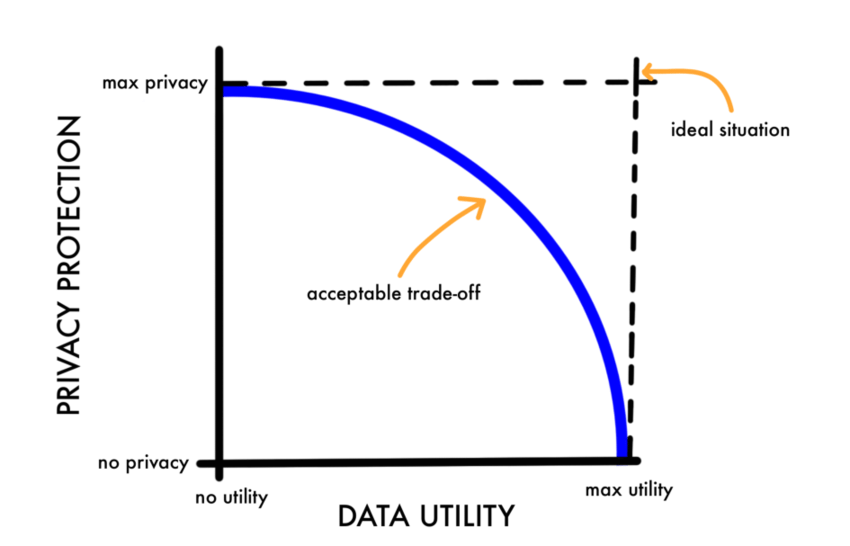
\includegraphics[width=0.8\textwidth]{images/Data-Privacy-Protection-versus-Data-Utility.png}
%    \caption{Illustration of the privacy-utility trade-off, from \citet{datasharing-implications}}
%    \label{fig:privacy-utility-tradeoff}
%\end{figure}

%\noindent This section introduces the concept of \textit{privacy filters}, which dynamically strip away attributes of exposed data in accordance with some predefined rules. A prototype middleware is developed which implements, along with macaroons, privacy filters. The concrete implementation is discussed in chapter \ref{cha:middleware}.

%Conceptually, this mechanism works as follows. Users load a number of privacy filter configuration files, which specify what transformations must happen to what datatype. Users can then specify how much privacy they want (in general, or for specific datatypes, see next section). When a request is received, \middleware{} checks the data type of the requested resource and the requested level of privacy. Subsequently, a number of transformations are applied to the data (as specified by the privacy filter configuration file), after which the transformed data is returned to the application. An example of what such a rewrite can look like is provided in figure \ref{fig:example-treatment-privacy-filter}.

%\noindent Privacy filters are represented by a configuration file for every filter. This configuration file describes the privacy tactics that must be applied to resources of a certain datatype. An example of such a configuration file is shown in the appendix, in listing \ref{listing:privacy-filter-kbc}.

%\subsection{Privacy levels}
%\label{sec:privacylevels}
%\noindent In order to provide an intuitive mechanism for selecting which data is transformed, the concept of privacy levels is introduced. Privacy levels form an abstraction above the concrete data transformations and \gls{PETs} that are applied to the data before it is passed on to the application. This ensures that non-technical users can use a privacy-enhancing middleware, without needing to understand the technical details of the technologies and tactics that are employed. 

% \middleware{} is configured with a default privacy level, but also supports specific privacy levels for certain data schemes. For example, a user could configure \middleware{} to use privacy level 2 by default, but privacy level 4 on bank transactions, since he does not want to expose this data. This makes the middleware more context-sensitive and allows for strong configurability. The privacy-utility trade-off can then also be taken into account for specific applications that need data with very high utility to deliver usable results. For every data scheme, an explanation should also be included which specifies concretely what will happen to the data under a certain privacy level.

% Another important aspect is that the developers of privacy filters for specific data schemes must be aware of what privacy levels map to what leakage or tactics. This is best determined by privacy experts as it is a very complex topic. However, appendix \ref{appendix:privacy-levels} shows an example of such a mapping that was used to guide the development of configuration files for the prototype of \middleware{}.



% \subsubsection{Supported transformations}
% Table \ref{table:supported-transformations} gives an overview of which transformations are currently supported in \middleware{}. The choice for supported transformations is mostly based on the discussion from section \ref{sec:transformation-approaches}. This section discussed a taxonomy of architectural tactics involving data transformations. Some tactics could not be mapped to an equivalent tactic in our middleware because the middleware works on a per-request basis. An example of this is the \textit{Select / Filter} tactic, which keeps a copy of the original data. The \textit{Aggregate} tactic was not applicable as \middleware{} does not support grouping data elements, as data is treated on a per-attribute basis. Similar arguments hold for other tactics that are not supported. The \textit{Perturbation} tactic is based on the \textit{Blur} tactic from table \ref{table:de-id-taxonomy}, but renamed to convey its applicability to numeric values. Similarly, \textit{Encrypt} is supported along with the similar \textit{Hash} tactic.

% \begin{table}[H]
\begin{center}
\begin{tabulary}{\textwidth}{p{0.20\textwidth}p{0.8\textwidth}}
\textbf{Transformation name} & \textbf{Description}                                                                                                                                                          \\ \hline
Remove               & The targeted and deliberate omission of PII from the data record or data set.                                                                                                 \\
Pseudonym            & The systematic replacement of direct identifiers with surrogates, whereby the mapping between surrogate and identity is kept separately.                                      \\
Perturbation         & The insertion of randomized noise into the values of the data to hide exact values                                                                                 \\
Random               & Tactics that involve the modification of PII attribute values/records by injecting artificial random elements.                                                                \\
Encrypt              & Using cryptographic means to encode the PII attribute values / records / datasets.                                                                                            \\
Hash                 & Using cryptographic hash functions to obfuscate the PII attribute values / records / datasets in a deterministic fashion.                                                                                            \\
\end{tabulary}
\caption{Overview of data transformations supported in \middleware{}}
\label{table:supported-transformations}
\end{center}
\end{table}
